\documentclass[11pt,a4paper]{article}

% Encodage et langue
\usepackage[utf8]{inputenc}
\usepackage[T1]{fontenc}
\usepackage[french]{babel}

% Maths et symboles
\usepackage{amsmath,amssymb,amsthm}

% Liens cliquables
\usepackage{hyperref}
\hypersetup{
  colorlinks=true,
  linkcolor=blue,
  urlcolor=blue,
  citecolor=blue,
  pdftitle={Spirale de l'inverse du temps},
  pdfauthor={Philippe Thomas Savard}
}

% Mise en page
\usepackage{geometry}
\geometry{margin=2.5cm}

% Pour insérer l'image
\usepackage{graphicx}

\title{Spirale de l'inverse du temps}
\author{Philippe Thomas Savard}
\date{Vingt avril deux mille vingt-six \\ Lévis, Chaudière-Appalaches, Canada}

\begin{document}

\maketitle

\section*{Mot de l'auteur}

Le présent document est rédigé avec une liberté de conscience complète et ne bénéficie d’aucun financement ni d’avantage de quelconque nature pour sa rédaction et sa création. Ce document est le fruit du travail d’un simple ouvrier qui n’a pas de formation du point de vue des mathématiques. Il est conçu avec un intérêt certain pour cette discipline et par plaisir intellectuel profond pour le sujet.

\begin{center}
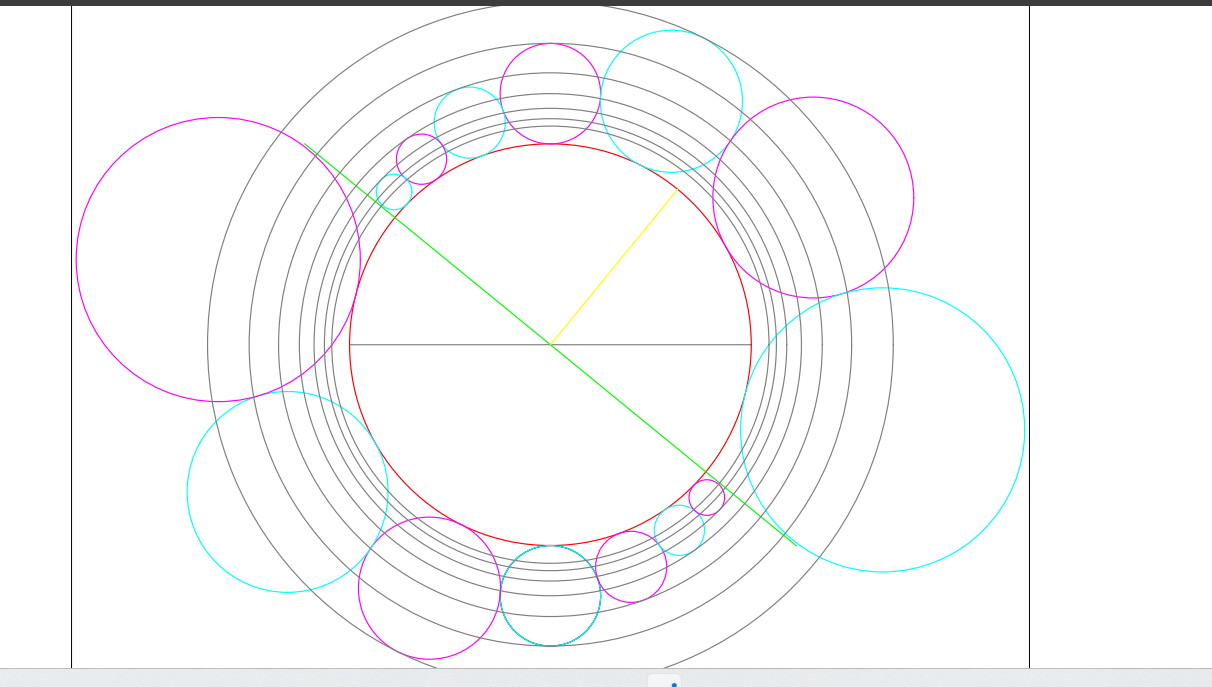
\includegraphics[width=0.75\textwidth]{spirale_inverse_temps.png}
\end{center}

\tableofcontents
\newpage

\section{Introduction}

La spirale de l’inverse du temps de Philippôt est un schéma géométrique qui inclut quinze disques tangents les uns aux autres. Pour décrire de manière plus complète, il s’agit d’un disque de rayon \(2\pi = 2\sqrt{10}\) sur lequel se trouvent deux fois une série de sept disques tangents au disque de \(2\sqrt{10}\).

Les sept disques tangents représentent les sept jours de la semaine, du dimanche au lundi et du lundi au dimanche. Le disque du centre est considéré comme étant le lundi à venir. Au bout de sept jours, les sept disques tangents à ce disque représentant le disque du lundi prochain sont donc situés sur le disque du futur.

Les aires de ces disques suivent la progression de la méthode de Philippôt et des termes de rapports \(1/k = 1/2\).

Exemple :


\[
\left( \frac{\sqrt{10} - (\sqrt{1.6})^{-3}/10}{\sqrt{10}} \times \frac{1}{2} \right)
= \frac{1}{128}
= 1 - \frac{\sqrt{10} - (\text{Aire du disque})}{\sqrt{10}}
\]



Les aires des huit disques :


\[
\begin{aligned}
A1 &= (\sqrt{1.6})^{-3}/10 \times 1/2 \\
A2 &= (\sqrt{1.6})^{-3}/10 \\
A3 &= 2 \times (\sqrt{1.6})^{-3}/10 \\
A4 &= 4 \times (\sqrt{1.6})^{-3}/10 \\
A5 &= 8 \times (\sqrt{1.6})^{-3}/10 \\
A6 &= 16 \times (\sqrt{1.6})^{-3}/10 \\
A7 &= 32 \times (\sqrt{1.6})^{-3}/10 \\
A8 &= 64 \times (\sqrt{1.6})^{-3}/10
\end{aligned}
\]



La valeur de la constante de l’inverse du temps :


\[
(\sqrt{1.6})^3 = 2.023857703
\]



\section{Description géométrique}

Les sept disques, de la droite vers la gauche pour la série du haut, vont du dimanche (rayon \(=\sqrt{1/2}\)), samedi (\(1/2\)), vendredi (\(\sqrt{1/8}\)), jeudi (\(1/4\)), mercredi (\(\sqrt{1/32}\)), mardi (\(1/8\)) et lundi (\(\sqrt{1/128}\)). Le disque du centre a un rayon de 1.

La spirale de l’inverse du temps est, pour l’auteur, une neuvième solution au problème d’Apollonius et au problème des contacts. L’auteur affirme que les sept disques sont également répartis sur \(\pi\) et que cette représentation permet une autre solution au problème des contacts d’Apollonius.

\section{Constante de l’inverse du temps}

Comme observé dans l’exemple précédent, les aires des disques — liées aux valeurs fractionnaires \(1/k = 1/2\) de la méthode de Philippôt — sont influencées par la constante de l’inverse du temps.

Cette constante est proposée par l’auteur dans \emph{L’univers est au carré} comme étant la valeur représentée par la Terre : \(40960\) km, correspondant au volume du diamètre de la Terre multiplié par \(10^{-2}\).



\[
\sqrt{40960} \times 10^{-2} = 2.023857703
\]



\section{Applications numériques}

C’est sur cette superficie que l’être humain accomplit son travail :  
\(1\) litre d’eau \(= 10^{79}\) bits d’information, sur un diamètre d’environ \(12000\) km.

La constante de l’inverse du temps \((\sqrt{1.6})^3 = 2.023857703\) sert à déterminer un ordre prédéterminé, comme :


\[
1/8.1 = 0.1234567901
\]



Exemple :


\[
\frac{6.48}{\sqrt{10}} = 2.049155924
\quad\Rightarrow\quad
\frac{(\sqrt{1.6})^3}{2.049155924} = 0.987654321
\]





\[
\frac{0.512 \times \sqrt{10}}{6.48/\sqrt{10}} = 0.7901234567901
\]



\section{Lien avec Cantor et les nombres premiers}

Selon l’auteur, cette manière de décomposer une séquence d’événements permet, à l’aide d’une version modifiée de la méthode de Cantor, de déterminer que les nombres premiers et composés sont uniformément répartis sur une surface \(1 \times 1\).

La droite unique du diamètre contient les nombres premiers positifs et négatifs.

Exemples :


\[
\begin{aligned}
100\% \times 0 &= 0 \\
101\% \times 0 &= -2 \\
102\% \times 0 &= 2 \\
103\% \times 0 &= -3 \\
104\% \times 0 &= 3 \\
105\% \times 0 &= -5 \\
107\% \times 0 &= 5
\end{aligned}
\]



\section{Exemples supplémentaires}



\[
(\sqrt{12.34567901}/(10/9))^2 = 10 \quad (1,0)
\]





\[
(\sqrt{23.456790123}/(10/9))^2 = 19 \quad (1,9)
\]





\[
(\sqrt{34.56790123}/(10/9))^2 = 28 \quad (2,8)
\]





\[
\sqrt{45.679012345}/(10/9) = 37 \quad (3,7)
\]



Autre exemple :



\[
1.234567901/2 = 0.6172839506
\]





\[
(\sqrt{0.6172839506}/(10/9))^2 = 0.5 \quad (0,5)
\]





\[
(\sqrt{0.172839506}/(10/9))^2 = 0.14 \quad (1,4)
\]





\[
(\sqrt{0.72839506}/(10/9))^2 = 0.59 \quad (5,9)
\]





\[
(\sqrt{0.2839506}/(10/9))^2 = 0.23 \quad (2,3)
\]





\[
(\sqrt{0.839506}/(10/9))^2 = 0.68 \quad (6,8)
\]



Ces exemples illustrent les usages possibles de la constante de l’inverse du temps.

\end{document}
